%%%%%%%%%%%%%%%%%%%%%%%%%%%%%%%%%%%%%%%%%
% Beamer Presentation
% LaTeX Template
% Version 1.0 (10/11/12)
%
% This template has been downloaded from:
% http://www.LaTeXTemplates.com
%
% License:
% CC BY-NC-SA 3.0 (http://creativecommons.org/licenses/by-nc-sa/3.0/)
%
%%%%%%%%%%%%%%%%%%%%%%%%%%%%%%%%%%%%%%%%%

%----------------------------------------------------------------------------------------
%	PACKAGES AND THEMES
%----------------------------------------------------------------------------------------

\documentclass{beamer}

\mode<presentation> {

% The Beamer class comes with a number of default slide themes
% which change the colors and layouts of slides. Below this is a list
% of all the themes, uncomment each in turn to see what they look like.

%\usetheme{default}
%\usetheme{AnnArbor}
%\usetheme{Antibes}
%\usetheme{Bergen}
%\usetheme{Berkeley}
%\usetheme{Berlin}
%\usetheme{Boadilla}
%\usetheme{CambridgeUS}
%\usetheme{Copenhagen}
%\usetheme{Darmstadt}
%\usetheme{Dresden}
%\usetheme{Frankfurt}
%\usetheme{Goettingen}
%\usetheme{Hannover}
%\usetheme{Ilmenau}
%\usetheme{JuanLesPins}
%\usetheme{Luebeck}
\usetheme{Madrid}
%\usetheme{Malmoe}
%\usetheme{Marburg}
%\usetheme{Montpellier}
%\usetheme{PaloAlto}
%\usetheme{Pittsburgh}
%\usetheme{Rochester}
%\usetheme{Singapore}
%\usetheme{Szeged}
%\usetheme{Warsaw}

% As well as themes, the Beamer class has a number of color themes
% for any slide theme. Uncomment each of these in turn to see how it
% changes the colors of your current slide theme.

%\usecolortheme{albatross}
%\usecolortheme{beaver}
%\usecolortheme{beetle}
%\usecolortheme{crane}
%\usecolortheme{dolphin}
%\usecolortheme{dove}
%\usecolortheme{fly}
%\usecolortheme{lily}
%\usecolortheme{orchid}
%\usecolortheme{rose}
%\usecolortheme{seagull}
%\usecolortheme{seahorse}
%\usecolortheme{whale}
%\usecolortheme{wolverine}

%\setbeamertemplate{footline} % To remove the footer line in all slides uncomment this line
%\setbeamertemplate{footline}[page number] % To replace the footer line in all slides with a simple slide count uncomment this line

\setbeamertemplate{navigation symbols}{} % To remove the navigation symbols from the bottom of all slides uncomment this line
}

\usepackage{graphicx} % Allows including images
\usepackage{booktabs} % Allows the use of \toprule, \midrule and \bottomrule in tables
\usepackage{verbatim}
%\usepackage{listings}
\usepackage{lipsum}
\usepackage{nicefrac}
\usepackage{alltt}

%----------------------------------------------------------------------------------------
%	TITLE PAGE
%----------------------------------------------------------------------------------------

\title[Tabby{XL}]{Tabby{XL}: Software Platform for Rule-Based Spreadsheet Data Extraction and Transformation*} % The short title appears at the bottom of every slide, the full title is only on the title page

\author[Shigarov et al.]{Alexey Shigarov \and Vasiliy Khristyuk \and \\ Andrey Mikhailov \and Viacheslav Paramonov} % Your name
\institute[ISDCT SB RAS] % Your institution as it will appear on the bottom of every slide, may be shorthand to save space
{
Matrosov Institute for System Dynamics and Control Theory,\\ Siberian Branch of the Russian Academy of Sciences \\ % Your institution for the title page
\medskip
\textit{shigarov@icc.ru} % Your email address
}

\small \date{October 2019}

\newif\ifshowtoc
\showtoctrue% toggles to show the toc
\AtBeginSection{%
\ifshowtoc
\begin{frame}
\frametitle{Table of Contents}
    \tableofcontents[currentsection, subsectionstyle=show/show/hide]
\end{frame}
\fi
}

\begin{document}

\begin{frame}
\titlepage % Print the title page as the first slide
\tiny\centerline{* This work was supported by the Russian Science Foundation, grant number 18-71-10001}
\end{frame}

%----------------------------------------------------------------------------------------
%	PRESENTATION SLIDES
%----------------------------------------------------------------------------------------

%------------------------------------------------
\section{Introduction} % Sections can be created in order to organize your presentation into discrete blocks, all sections and subsections are automatically printed in the table of contents as an overview of the talk
%------------------------------------------------

\subsection{Motivation}

\begin{frame}
\frametitle{Motivation}
\begin{itemize}
\item About arbitrary spreadsheet tables 
\begin{itemize}
	\item A large volume of valuable data for science and business applications
	\item A big variety of layout, style, and content features
	\item Human-centeredness (incorrect structure and messy content)
	\item No explicit semantics for interpretation by computers
\end{itemize}
\bigskip
\item Challenges
\begin{itemize}
	\item How to extract tables from worksheets
	\item How to recognize and correct cell structure anomalies
	\item How to recover semantics needed for the automatic interpretation
	\item How to conceptualize extracted data by using external vocabularies
\end{itemize}
\end{itemize}
\end{frame}

\subsection{Background}

\begin{frame}
\frametitle{Background}
\emph{Table understanding} \cite{Hurst2001} includes the following tasks
\bigskip

\begin{enumerate}
	\item \textbf{Extraction} --- detecting a table and recognizing the physical structure of its cells 
	\item \textbf{Role analysis} --- extracting functional data items from cell content
	\item \textbf{Structural analysis} --- recovering internal relationships between extracted functional data items
	\item \textbf{Interpretation} --- linking extracted functional data items with external vocabularies (general-purpose or domain-specific ontologies)
\end{enumerate}

\end{frame}

\begin{frame}
\frametitle{Background}
The related issues of the \emph{table analysis and interpretation}
\bigskip

{\footnotesize
\begin{itemize}
\item \textbf{Layout properties} \cite{Koci2017,Chen2017,Dou2018}
\item \textbf{Code smells and formulas} \cite{Hermans2015,Dou2017,Barowy2018,Koch2019}
\item \textbf{Programming by examples} \cite{Barowy2015,Singh2016,Jin2017}
\item \textbf{Data model inference} \cite{Amalfitano2015,Cunha2015,Cunha2016}
\item \textbf{Linked Open Data} \cite{Ritze2017,Zhang2017}
\item \textbf{Domain-specific models} \cite{Vos2017,Cao2017,Swidan2017}
\item \textbf{Rule-based programming} \cite{Yang2017,Shigarov2017,Yang2018}
\end{itemize}
}

\end{frame}

\begin{frame}
\frametitle{Background}
The projects with goals similar to ours
\bigskip

\begin{enumerate}
\item \footnotesize{\textbf{TANGO}\footnote{\url{https://tango.byu.edu}} (Data Extraction Group, Brigham Young University) \textit{2005 -- 2016}}
\begin{itemize}
\item \scriptsize{Heuristics-based role analysis (pre-defined functional cell regions) \cite{Embley2016}}
\end{itemize}
\item \footnotesize{\textbf{Senbazuru}\footnote{\url{http://dbgroup.eecs.umich.edu/project/sheets}} (Database Research Group, University of Michigan) \textit{2013 -- 2017}}
\begin{itemize}
\item \scriptsize{ML-based role analysis (pre-defined functional cell regions) \cite{Chen2016}}
\item \scriptsize{ML-based structural analysis (pre-defined layout properties of the header hierarchy) \cite{Chen2016}}
\end{itemize}
\item \footnotesize{\textbf{DeExcelerator}\footnote{\url{https://wwwdb.inf.tu-dresden.de/research-projects/deexcelarator}} (Dresden Database Systems Group, TU Dresden) \textit{2013 -- 2019}}
\begin{itemize}
\item \scriptsize{ML-based layout identification}~\cite{Koci2016}
\item \scriptsize{Heuristics-based role and structural analysis (pre-defined functional cell regions) \cite{Koci2017,Koci2018}} 
\end{itemize}
\end{enumerate}

\end{frame}

\subsection{Contribution}

\begin{frame}
\frametitle{Contribution}

\small TabbyXL is a software platform aiming at the development and execution of rule-based programs for spreadsheet data extraction and transformation from arbitrary (\textit{a}) to relational tables (\textit{b})

\begin{columns}[c] % The "c" option specifies centered vertical alignment while the "t" option is used for top vertical alignment

\column{.4\textwidth} % Left column and width

\begin{block}{\small Novelty}
\begin{itemize}
\item \small Table object model assigning roles to data items, not cell
\item \small CRL, domain-specific language to express user-defined rules for table analysis and interpretation
\item \small CRL-to-Java translator to synthesize executable programs for spreadsheet data transformation
\end{itemize}
\end{block}

\column{.6\textwidth} % Right column and width
\begin{figure}
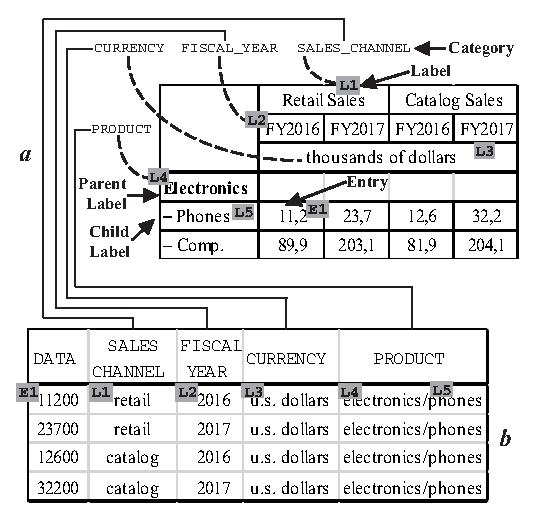
\includegraphics[width=0.85\linewidth]{intro}
\end{figure}

\end{columns}

\end{frame}

\section{Approach}

\subsection{User-Defined Rules}

\begin{frame}
\frametitle{User-Defined Rules}
\begin{itemize}
\item The user-defined rules map the physical structure into the logical structure of a table 
\begin{itemize}
\item \textbf{WHEN-part} queries facts about the structure by using constraints
\item \textbf{THEN-part} modifies available facts and asserted new ones
\end{itemize}
\item The facts are represented by items of the \emph{table object model}
\item The rules can be expressed in a rule-based language 
(e.g. Drools\footnote{\url{https://www.drools.org}}, Jess\footnote{\url{https://jessrules.com}}, or CRL\footnote{\url{https://github.com/tabbydoc/tabbyxl/wiki/crl-language}})
\end{itemize}
\end{frame}

\subsection{Table Object Model}

\begin{frame}
\frametitle{Table Object Model}

\begin{columns}[c] % The "c" option specifies centered vertical alignment while the "t" option is used for top vertical alignment

\column{.4\textwidth} % Left column and width

\begin{block}{\small Physical Layer}
\small Cells characterized by layout, style, and content features
\end{block}
\begin{block}{\small Logical Layer}
\small Functional data items and their relationships: 
\begin{itemize}
	\item \small entries (values)
	\item \small labels (keys)
	\item \small categories (concepts)
	\item \small entry-label pairs
	\item \small label-label pairs
	\item \small label-category pairs
\end{itemize}
\end{block}

\column{.6\textwidth} % Right column and width
\begin{figure}
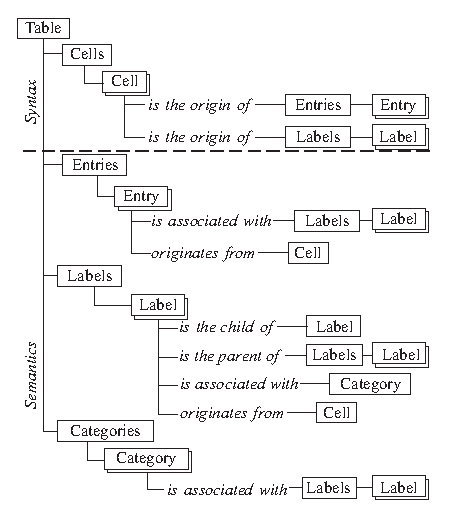
\includegraphics[width=0.85\linewidth]{tom}
\end{figure}

\end{columns}

\end{frame}

\begin{frame}
\frametitle{CRL Grammar}

\begin{figure}
\includegraphics[width=0.75\linewidth]{bnf}	
\end{figure}
\end{frame}

\subsection{Cell Cleansing}

\begin{frame}[fragile]
\frametitle{Cell Cleansing}
The actions correct an inaccurate layout and content of a hand-coded table
\begin{itemize}
	\item \alert{<merge>} combines two adjacent cells when they share one border
	\item \alert{<split>} divides a merged cell that spans $n$-tiles (row-column intersections) into $n$-cells
	\item \alert{<set text>} modifies a textual content of a cell
	\item \alert{<set indent>} modifies a text indentation of a cell
\end{itemize}

\footnotesize{
\begin{example}
\begin{alltt}
\textbf{when}
  \textbf{cell} corner: cl == 1, rt == 1, blank
  \textbf{cell} c: cl > corner.cr, rt > corner.rb
\textbf{then}
  \textbf{split} c
\end{alltt}
\end{example}
}

\end{frame}

\subsection{Role Analysis}

\begin{frame}[fragile]
\frametitle{Role Analysis}
The actions recover entries and labels as functional data items presented in a table
\begin{itemize}
	\item \alert{<set mark>} annotates a cell with a user-defined tag that can be used in subsequent table analysis
	\item \alert{<new entry>} (\alert{<new label>}) creates an entry (label) from a cell content with the use of an optional string processing
\end{itemize}

\footnotesize{
\begin{example}
\begin{alltt}
\textbf{when}
  \textbf{cell} corner: cl == 1, rt == 1, blank
  \textbf{cell} c: cl > corner.cr, rt > corner.rb
\textbf{then}
  \textbf{new entry} c
\end{alltt}
\end{example}
}

\end{frame}

\subsection{Structural Analysis}

\begin{frame}[fragile]
\frametitle{Structural Analysis}
The actions recover pairs of two kinds: entry-label and label-label
\begin{itemize}
	\item \alert{<add label>} associates an entry with a label
	\item \alert{<set parent>} binds two labels as a parent and its child
\end{itemize}

\footnotesize{
\begin{example}
\begin{alltt}
\textbf{when}
  \textbf{cell} c1: cl == 1
  \textbf{cell} c2: cl == 1, rt > c1.rt, indent == c1.indent + 2
  \textbf{no cells}: cl == 1, rt > $c1.rt, rt < $c2.rt, indent == $c1.indent
\textbf{then}
  \textbf{set parent} c1.label \textbf{to} c2.label
\end{alltt}
\end{example}
}

\end{frame}

\subsection{Interpretation}

\begin{frame}[fragile]
\frametitle{Interpretation}
The actions serve to recover label-category pairs
\begin{itemize}
	\item \alert{<set category>} associates a label with a category
	\item \alert{<group>} places two labels to one group that can be considered as an undefined category
\end{itemize}

\footnotesize{
\begin{example}
\begin{alltt}
\textbf{when}
  \textbf{label} l1: cell.mark == "stub"
  \textbf{label} l2: cell.mark == "stub", cell.rt == l1.cell.rt
\textbf{then}
  \textbf{group} l1 \textbf{with} l2
\end{alltt}
\end{example}
}

\end{frame}

\subsection{Illustrative Example}

\begin{frame}
\frametitle{Illustrative Example}

\scriptsize{The transformation of arbitrary tables with the same layout features (\textit{a} and \textit{c}) to their canonicalized versions (\textit{b} and \textit{d})}
\begin{figure}
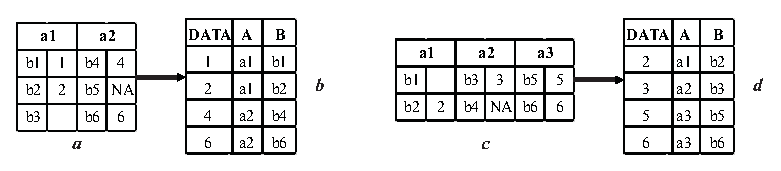
\includegraphics[width=0.7\linewidth]{illustrative_example}	
\end{figure}

\scriptsize{The ruleset for the cell cleansing (\textit{a}), role analysis (\textit{b}, \textit{c}), structural analysis (\textit{d}, \textit{e}), and interpretation (\textit{f}, \textit{g})}
\begin{figure}
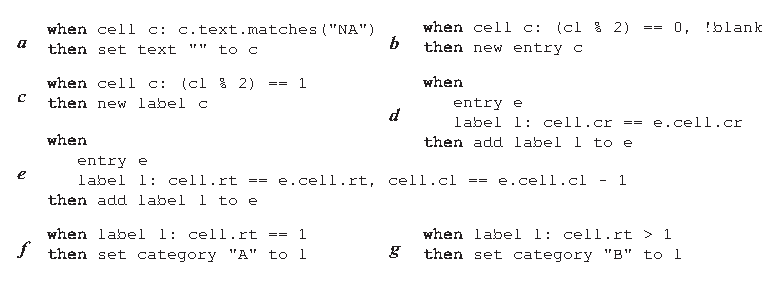
\includegraphics[width=0.75\linewidth]{illustrative_example_rules}
\end{figure}

\tiny{This example is reproducible at \url{https://codeocean.com/capsule/5326436}}

\end{frame}

\section{Software Platform}

\subsection{Architecture}

\begin{frame}
\frametitle{Architecture}
\begin{figure}
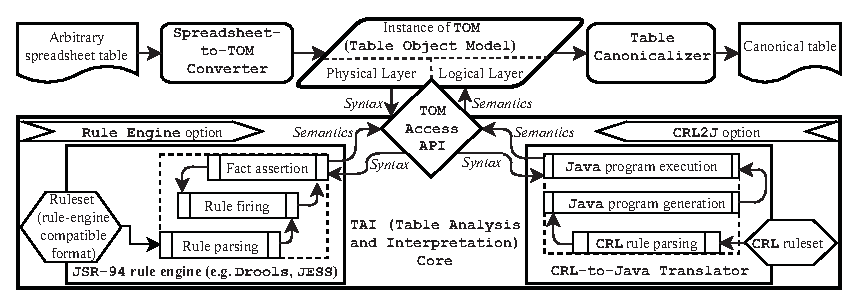
\includegraphics[width=1.0\linewidth]{architecture}
\end{figure}
\hspace*{\fill} \textbf{Two options are provided} \hspace*{\fill}
\begin{columns}
\column{.5\textwidth}
\begin{block}{\small Rule Engine option}
\small Executing a ruleset in an appropriate format with a JSR-94 compatible rule engine (e.g. Drools, Jess)
\end{block}
\column{.4\textwidth}
\begin{block}{\small CRL2J option}
\small Translating a ruleset expressed in CRL to an executable Java program
\end{block}
\end{columns}

\end{frame}

\subsection{CRL2J Translation}

\begin{frame}
\frametitle{CRL2J Translation}
\begin{columns}[t]
\column{.55\textwidth}
\small Workflow for generating a Maven-project of a spreadsheet data transformation program
\begin{figure}
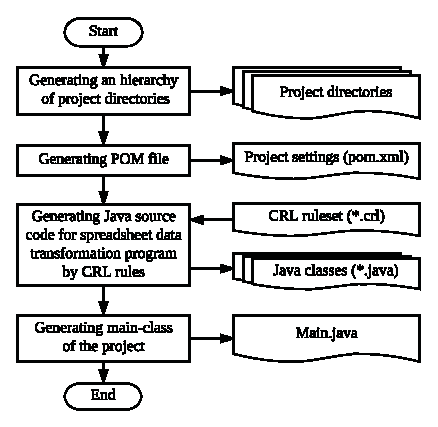
\includegraphics[width=0.95\linewidth]{crl2j_wf_part1}	
\end{figure}

\column{.05\textwidth}
\\~\\

\column{.4\textwidth}
\small Workflow for translating a CRL ruleset to Java source code
\begin{figure}
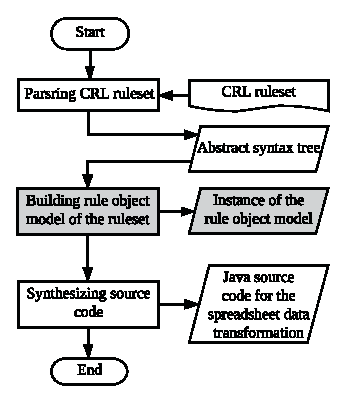
\includegraphics[width=0.95\linewidth]{crl2j_wf_part2}	
\end{figure}
\end{columns}
\end{frame}

\begin{frame}
\frametitle{CRL2J Translation}

\begin{columns}
\column{.3\textwidth}
\small{\centerline{In the Workflow}}

\begin{figure}
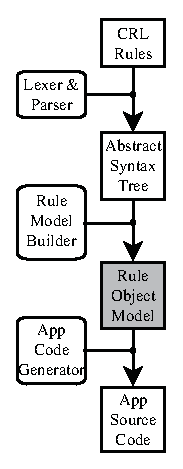
\includegraphics[width=0.65\linewidth]{rom_in_wf.eps}	
\end{figure}

\column{.7\textwidth}
\small{\centerline{Rule Object Model}}

\begin{figure}
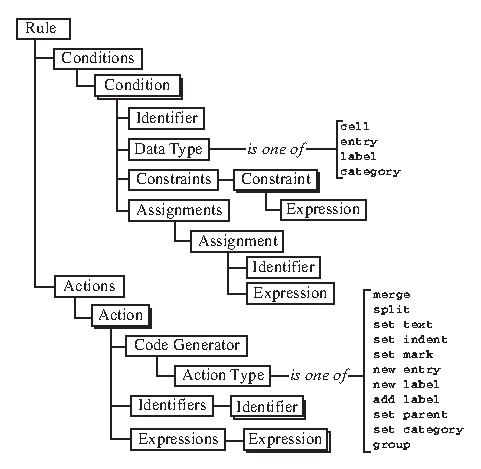
\includegraphics[width=0.8\linewidth]{rulemodel}	
\end{figure}
\end{columns}

\end{frame}

\begin{frame}[fragile] % Need to use the fragile option when verbatim is used in the slide
\frametitle{CRL2J Translation}

\footnotesize{
\begin{example}[Source Rule]
\begin{alltt}
\textbf{when}
  \textbf{cell} corner: cl == 1, rt == 1, blank
  \textbf{cell} c: cl > corner.cr, rt > corner.rb, ! marked
\textbf{then}
  \textbf{set mark} "@entry" \textbf{to} c
  \textbf{new entry} c
\end{alltt}
\end{example}
}
\footnotesize{
\begin{example}[Fragment of the Generated Java Code]
\begin{alltt}
...
Iterator<CCell> iterator1 = getTable().getCells();
\textbf{while} (iterator1.hasNext()) \{
  corner = iterator1.next();
  \textbf{if} ((corner.getCl() == 1) && (corner.getRt() == 1) && ...
    Iterator<CCell> iterator2 = getTable().getCells();
    \textbf{while} (iterator2.hasNext()) \{
...
\end{alltt}
\end{example}
}
\end{frame}

%------------------------------------------------

\section{Empirical Results}

\subsection{Performance Evaluation}

\begin{frame}
\frametitle{Performance Evaluation}

\small{The results of the transformation of 200 tables of Troy200 dataset \cite{Nagy2016}}

\footnotesize{
\begin{table}
		\centering
		    \bgroup
        \def\arraystretch{1.5}
				\begin{tabular}{|l|c|c|c|c|}
						\hline
														& \multicolumn{2}{|c|}{Role analysis} & \multicolumn{2}{|c|}{Structural analysis} \\ 
														\cline{2-5} 
														& \multicolumn{4}{|c|}{Type of instances} \\ 
														\cline{2-5} 
			            Metrics   & entries                      & labels                     & entry-label pairs            & label-label pairs  \\
			      \hline
			            Recall    & 0.9813 $\frac{16602}{16918}$ & 0.9965 $\frac{4842}{4859}$ & 0.9773 $\frac{34270}{35066}$ & 0.9389 $\frac{1951}{2078}$ \\
			            Precision & 0.9996 $\frac{16602}{16609}$ & 0.9364 $\frac{4842}{5171}$ & 0.9965 $\frac{34270}{34389}$ & 0.9784 $\frac{1951}{1994}$ \\
									$F$-score & 0.9904                       & 0.9655                     & 0.9868                       & 0.9582                     \\
			      \hline
		    \end{tabular}
				\egroup
\end{table}
}

\begin{block}{\small Metrics}
\footnotesize{
\begin{equation*}
\begin{aligned}[c]
\mbox{recall} = \nicefrac{\left|R \cap S\right|}{\left|S\right|}
\end{aligned}
\quad
\begin{aligned}[c]
\mbox{precision} = \nicefrac{\left|R \cap S\right|}{\left|R\right|}
\end{aligned}
\end{equation*}
}
\scriptsize{\centerline{$S$ is a set of instances in a source table, $R$ is a set of instances in its canonical form}}
\end{block}

\tiny All data and steps to reproduce the results are available at \url{http://dx.doi.org/10.17632/ydcr7mcrtp.5}

\end{frame}

\begin{frame}
\frametitle{Performance Evaluation}

\small{The comparison of the running time by using TabbyXL with three different options for transforming 200 tables of Troy200 dataset \cite{Nagy2016}}
\begin{table}
		\centering
		    \bgroup
        \def\arraystretch{1.5}
				\begin{tabular}{|l|c|c|c|}
						\hline
									Running time of             & CRL2J   & Drools  & Jess     \\ 
						\hline														
									Ruleset preparation ($t_1$) & 2108* ms & $1711^\dagger$ ms & $432^\dagger$  ms \\
                  Ruleset execution ($t_2$)   & 367** ms & $1974^\ddagger$ ms & $4149^\ddagger$ ms \\
			      \hline
		    \end{tabular}
				\egroup
\end{table}

\scriptsize{
* $t_1$ --- a time of parsing and compiling the original ruleset into a Java program \\
** $t_2$ --- a time of executing the generated Java program
\\~\\
$^\dagger$ $t_1$ --- a time of parsing the original ruleset and adding the result into a rule engine session \\
$^\ddagger$ $t_2$ --- a time of asserting facts into the working memory and matching rules against the facts
\\~\\
For testing, we used 3.2 GHz 4-core CPU
}


\end{frame}

\subsection{Comparison with Others}

\begin{frame}
\frametitle{Comparison with Others}

\small{
\begin{block}{Role Analysis}
\begin{itemize}
\item \emph{Contest task}: The segmentation of a table into typical functional cell regions
\item \emph{Testing dataset}: Troy200  \cite{Nagy2016}
\item \emph{Contestant}: MIPS (TANGO) \cite{Embley2016}
\item \emph{Accuracy}: MIPS (TANGO) --- \textbf{0.9899} vs. TabbyXL --- \textbf{0.9950}
\end{itemize}
\end{block}

\begin{block}{Structural Analysis}
\begin{itemize}
	\item \emph{Contest task}: The extraction of header hierarchies from tables
	\item \emph{Testing dataset}: A random subset of SAUS\footnote{\url{http://dbgroup.eecs.umich.edu/project/sheets/datasets.html}}
	\item \emph{Contestant}: Senbazuru \cite{Chen2014}
	\item $F$\emph{-score}: Senbazuru --- \textbf{0.8860} vs. TabbyXL --- \textbf{0.8657}
\end{itemize}
\end{block}
}
\end{frame}

\section{Application Experience}

\begin{frame}
\frametitle{Application Experience}
Populating a web-based statistical atlas of the Irkutsk region --- (\textit{b}) via extracting data from government statistical reports --- (\textit{a})
\begin{figure}
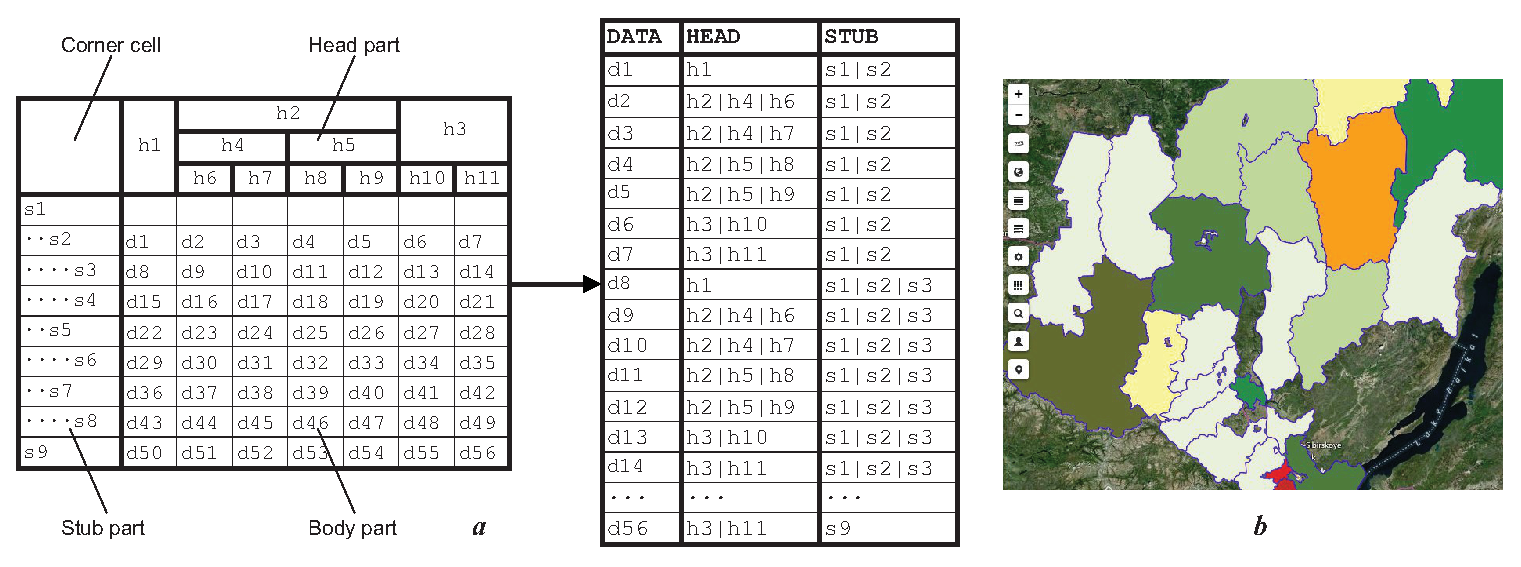
\includegraphics[width=1\linewidth]{application1}	
\end{figure}
\tiny{The more detail can be found at \url{https://github.com/tabbydoc/tabbyxl/wiki/statistical-atlas}}
\end{frame}

\begin{frame}
\frametitle{Application Experience}
Generating conceptual models --- (\textit{b}) from arbitrary tables presented in industrial safety inspection reports --- (\textit{a})
\begin{figure}
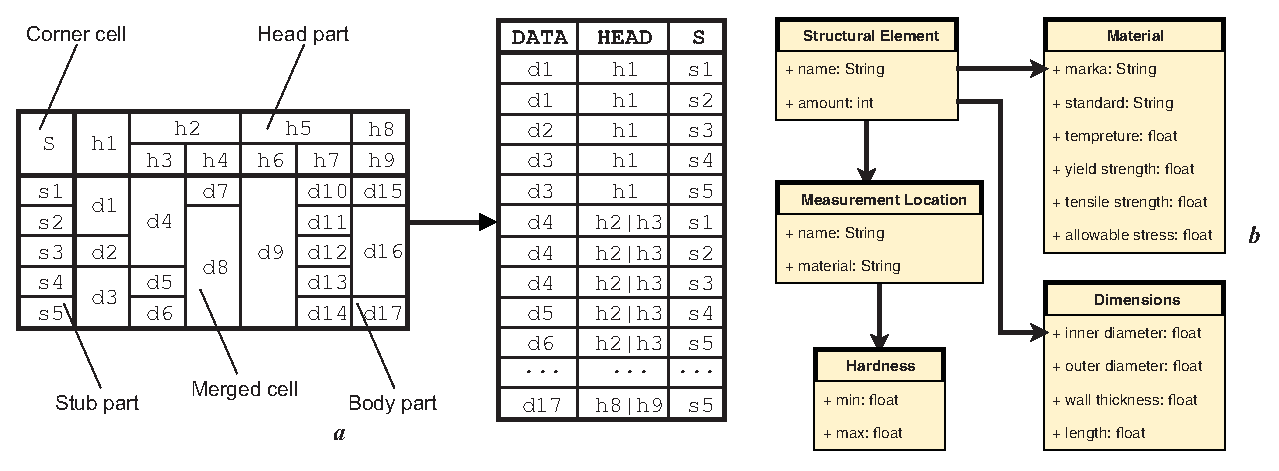
\includegraphics[width=1\linewidth]{application2}	
\end{figure}
\tiny{The more detail can be found at \url{https://github.com/tabbydoc/tabbyxl/wiki/industrial-safety-inspection}}
\end{frame}

\section{Conclusions \& Further Work}

\begin{frame}
\frametitle{Conclusions \& Further Work}

\begin{itemize}
\item Impact on software development for spreadsheet data management
\begin{itemize}
\item Table object model associating functional roles with data items
\item Table analysis and interpretation driven by user-defined rules
\item Formulated actions to recover missing semantics of arbitrary tables
\item Translation of rules to executable spreadsheet transformation programs
\end{itemize}
\medskip
\item Limitations
\begin{itemize}
\item The inaccurate cell structure prevents the table analysis
\item The very limited interpretation (without external vocabularies)
\end{itemize}
\medskip
\item Further work
\begin{itemize}
\item Rearrangement of cell structure by using visual (human-readable) cells
\item Detecting derived data by spreadsheet formulas
\item Enriching the table analysis by named entity recognition 
\item Linking extracted data items with LOD cloud
\end{itemize}
\end{itemize}

\end{frame}

\section{References}

\begin{frame}[allowframebreaks]
\frametitle{References}
\tiny
\bibliographystyle{apalike}
\bibliography{mybibfile}
\end{frame}

\begin{frame}
\Huge{\centerline{Thanks}}
\bigskip
\footnotesize{\centerline{Read more about the project at}}
\scriptsize{\centerline{\url{http://td.icc.ru}}}

\bigskip
\footnotesize{\centerline{The project source code is available at}}
\scriptsize{\centerline{\url{https://github.com/tabbydoc/tabbyxl}}}
\end{frame}

%----------------------------------------------------------------------------------------

\end{document} 